
\documentclass{beamer}
\usetheme{Singapore}
\usepackage[dark,accent=blue]{../../assets/beamercolorthemesolarized}
\setbeamertemplate{navigation symbols}{\insertframenumber}
\setbeamercolor{navigation symbols}{fg = solarizedAccent}
\setbeamerfont{navigation symbols}{size = \tiny}

\usepackage{helvet, hyperref, tikz}
\usetikzlibrary{arrows.meta, shapes.geometric}
\tikzset{>={To[length=3mm,width=3mm]}}

\graphicspath{{..}}

\title{Winning baseball games by\\solving statistics puzzles}
\author{Scott Powers}
\date{TAMIDS Seminar Series\\February 16, 2026}
\begin{document}

  \begin{frame}
      \maketitle
      \vfill\hfill
\includegraphics[width = 4cm]{../../assets/rice_logo_white.png}
  \end{frame}

  \begin{frame}{What is Sport Analytics?}
    
\includegraphics[width = \textwidth]{images/sport_analytics.jpg}
  \end{frame}

  \begin{frame}{Books about Baseball Teams Using Analytics to Win}
    \begin{columns}
      \begin{column}{0.25\textwidth}
        \centering
        
\includegraphics[width = \textwidth]{images/books/moneyball.jpg}\\
        ~\\
        2002\\ Oakland\\ Athletics
      \end{column}
      \begin{column}{0.25\textwidth}
        \centering
        
\includegraphics[width = \textwidth]{images/books/the_extra_two.jpg}\\
        ~\\
        2008\\ Tampa Bay\\ Rays
      \end{column}
      \begin{column}{0.25\textwidth}
        \centering
        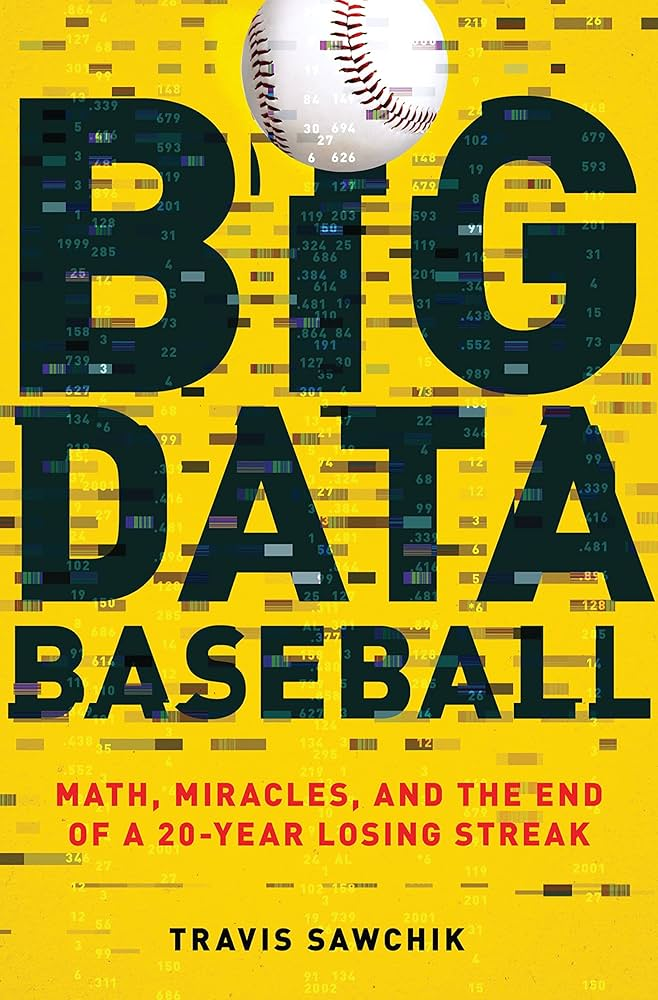
\includegraphics[width = \textwidth]{images/books/big_data_baseball.jpg}\\
        ~\\
        2013\\ Pittsburgh\\ Pirates
      \end{column}
      \begin{column}{0.25\textwidth}
        \centering
        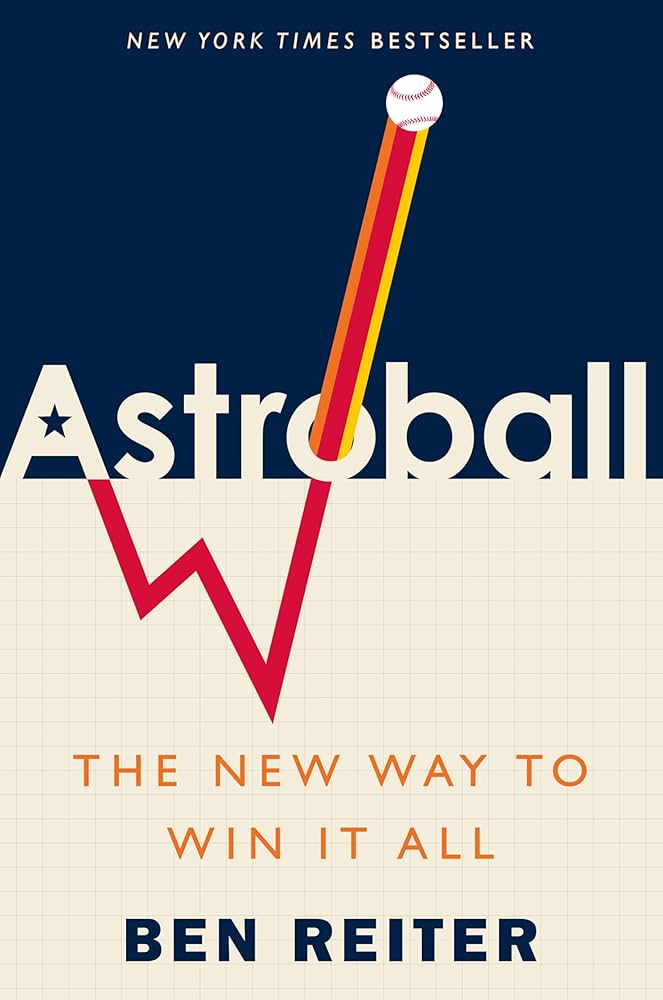
\includegraphics[width = \textwidth]{images/books/astroball.jpg}\\
        ~\\
        2017\\ Houston\\ Astros
      \end{column}
    \end{columns}
  \end{frame}

  \begin{frame}{MLB R\&D Staff Sizes (according to Reddit)}
    \begin{columns}
      \begin{column}{0.55\textwidth}
        \centering
        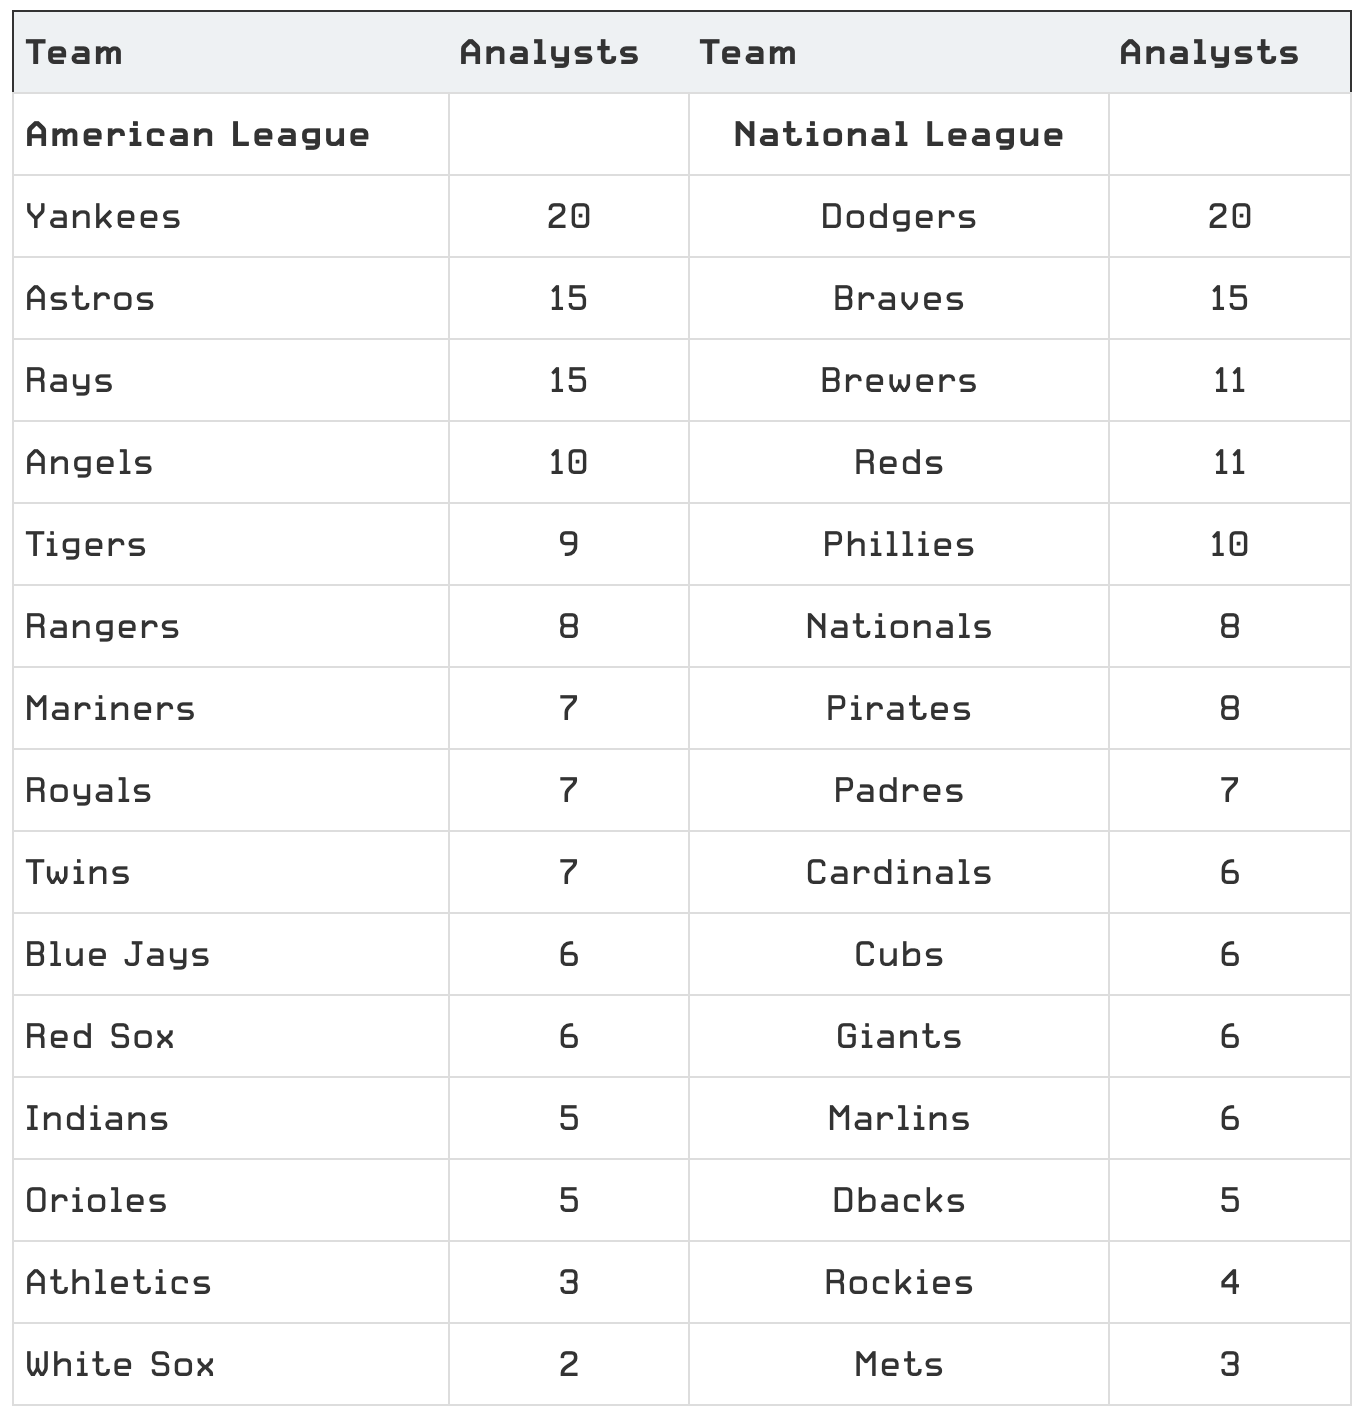
\includegraphics[width=\textwidth]{images/staff_2018.png}\\
        2018
      \end{column}
      \begin{column}{0.45\textwidth}
        \centering
        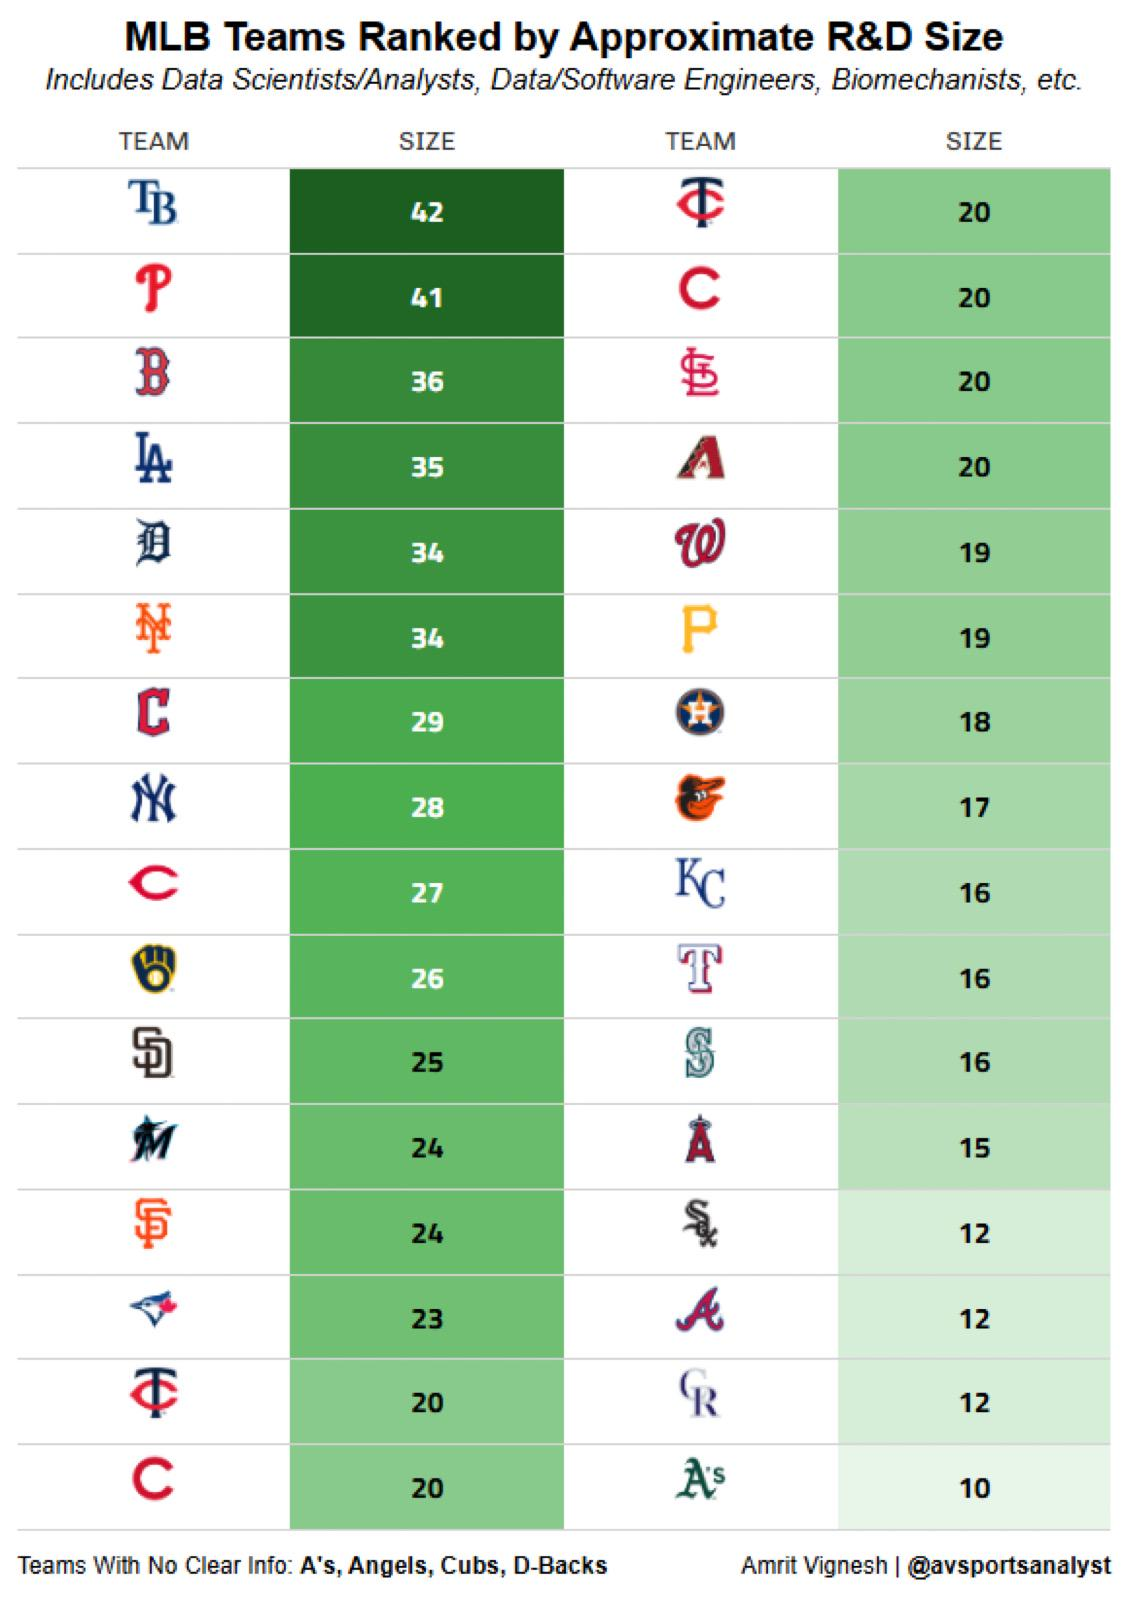
\includegraphics[width=\textwidth]{images/staff_2025.jpeg}\\
        2025
      \end{column}
    \end{columns}
  \end{frame}

  \begin{frame}{What are they all doing?}
    \centering
    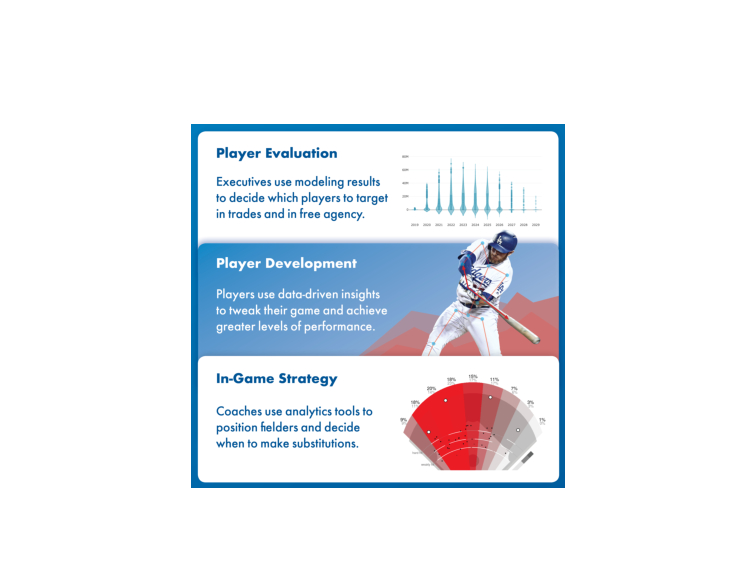
\includegraphics[height=0.8\textheight]{images/applications.pdf}
  \end{frame}
  
  \begin{frame}{Three Puzzles}
    \begin{columns}
      \begin{column}{0.46\textwidth}
        \begin{enumerate}
          \item[I:] How far should you stray\\from first base?
          \vspace{1.5cm}
          \item[II:] Should you just swing\\as hard as you can? 
          \vspace{1.5cm}
          \item[III:] What does a pitch\\tell you about a pitcher?
        \end{enumerate}
      \end{column}
      \begin{column}{0.4\textwidth}
        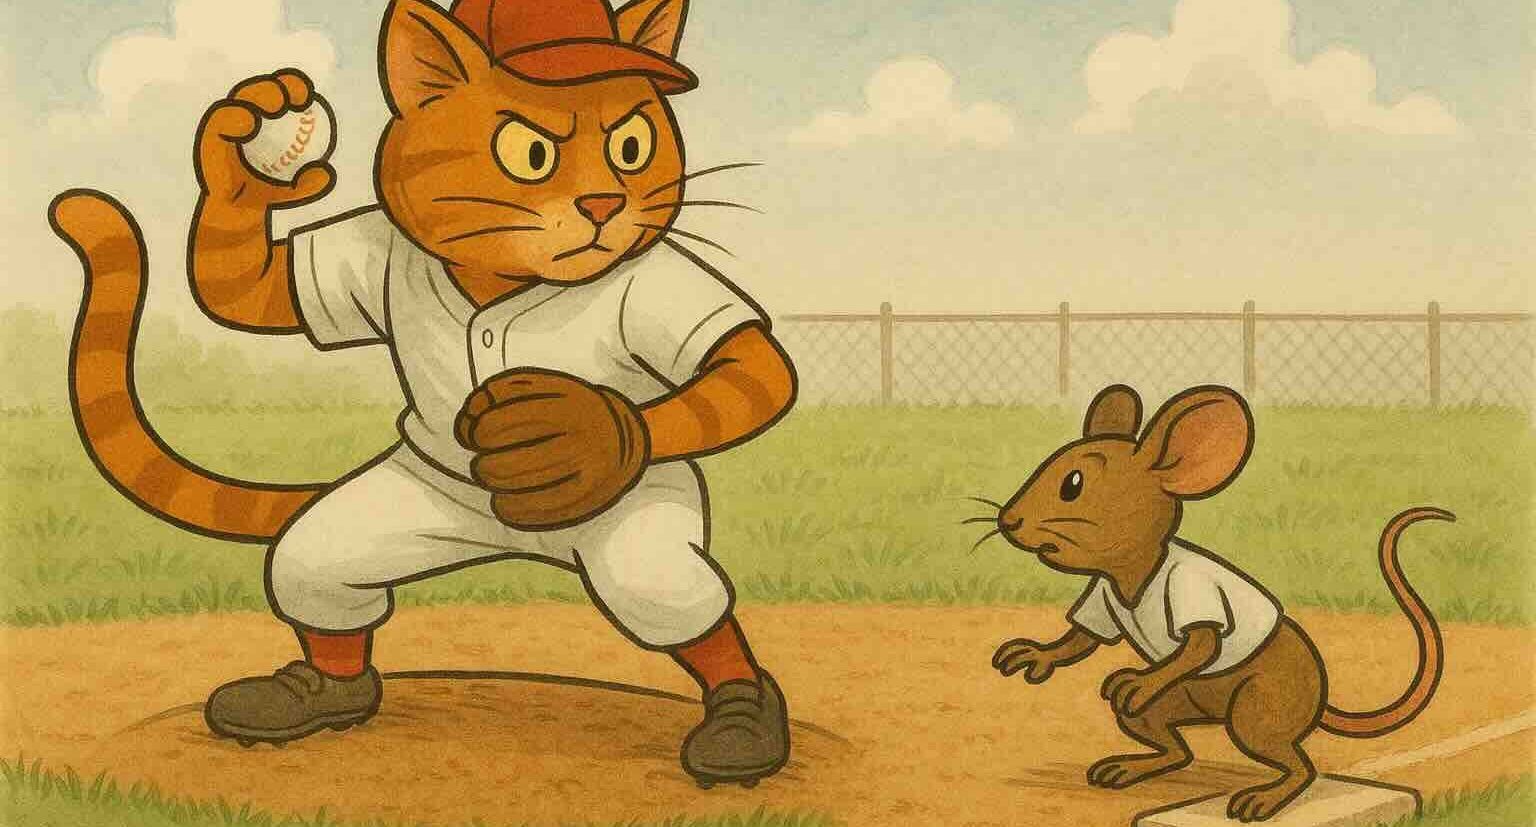
\includegraphics[width = \textwidth]{images/cat_and_mouse.jpg}\\
        ~\\
        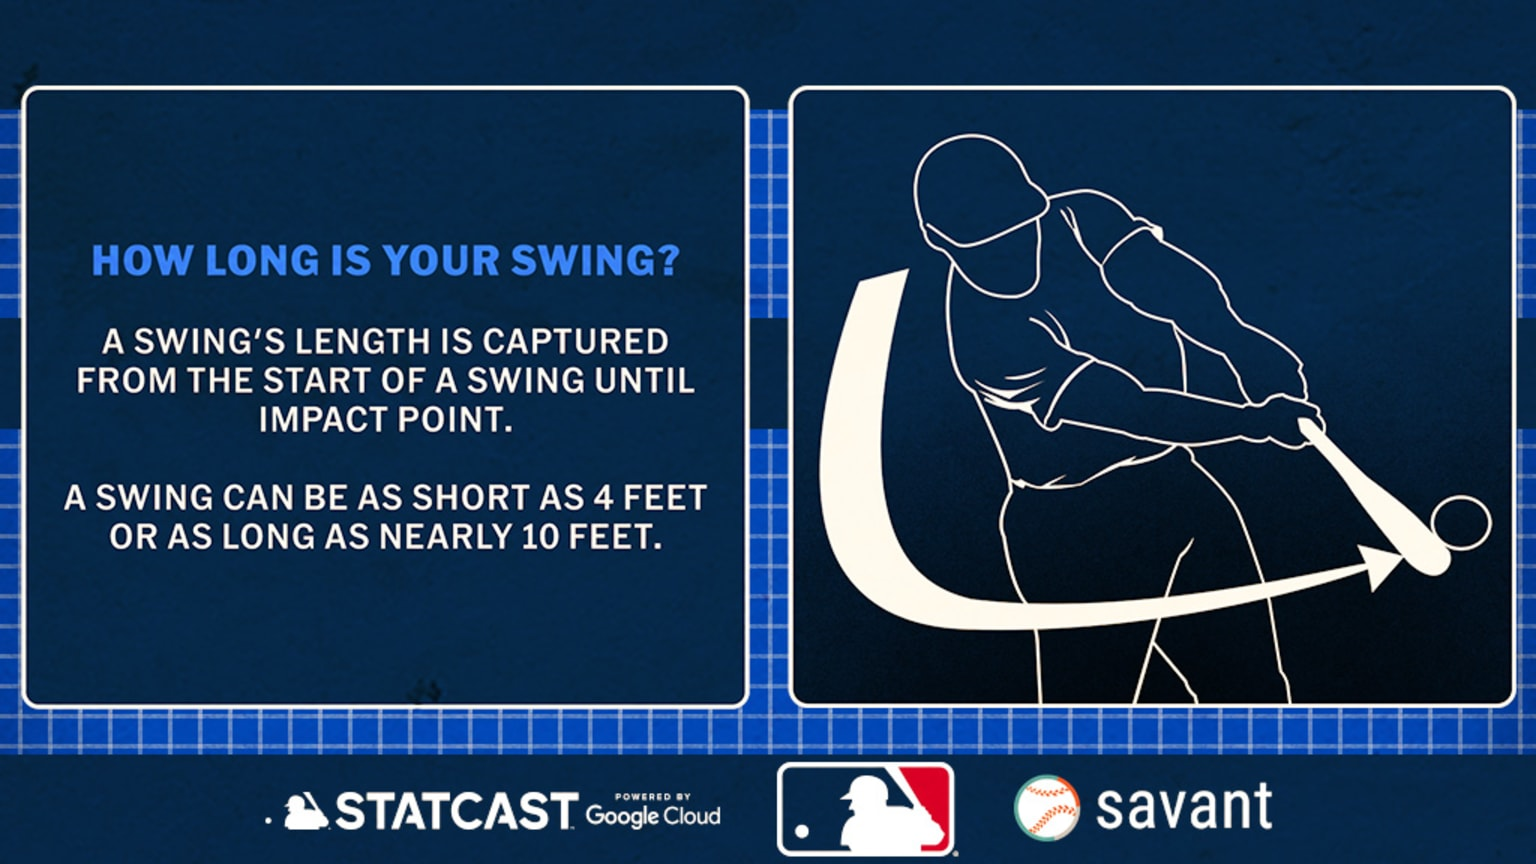
\includegraphics[width = \textwidth]{images/swing_length.jpg}\\
        ~\\
        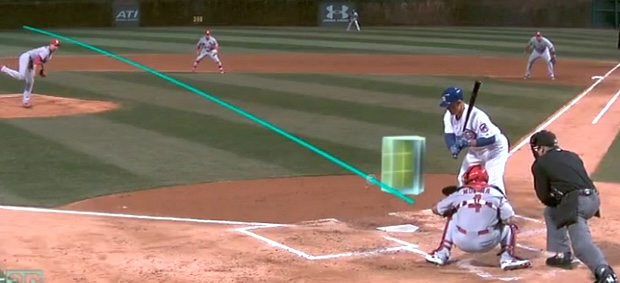
\includegraphics[width = \textwidth]{images/pitch_tracking.jpg}
      \end{column}
    \end{columns}
  \end{frame}

  \begin{frame}{How far should you stray from first base?}
    
\includegraphics[height=0.5in]{images/collaborators/ramani.jpg}
    \alert{Sivaramakrishnan Ramani}, Rice University\\
    ~\\
    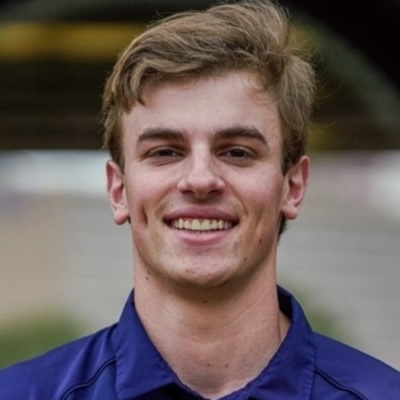
\includegraphics[height=0.5in]{images/collaborators/hahn.jpg}
    \alert{Jacob Hahn}, Rice University $\rightarrow$ Chicago Cubs\\
    ~\\
    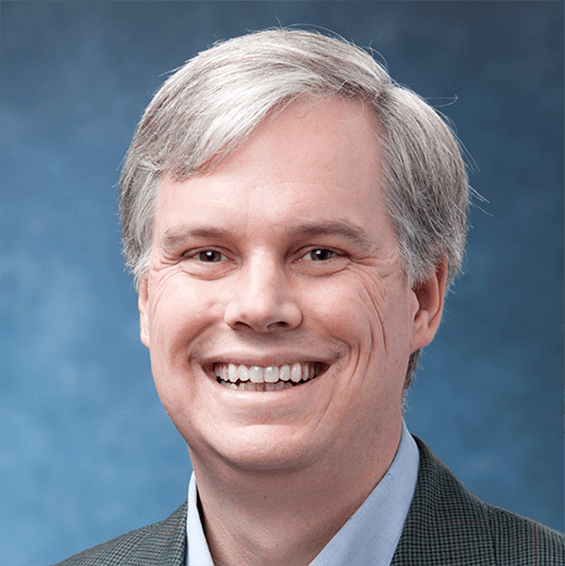
\includegraphics[height=0.5in]{images/collaborators/schaefer.png}
    \alert{Andrew Schaefer}, Rice University\\
    ~\\
    \small Powers S, Ramani S, Hahn J, Schaefer AJ (2026)\\
    ``Lead distance under a pickoff limit in Major League Baseball: A sequential game model''\\
    \href{https://arxiv.org/abs/2601.15608}{arXiv:2601.15608}
  \end{frame}

  \begin{frame}{Background}
    In 2023, MLB limited the pitcher to \alert{\bf 3 pickoff attempts}
    \begin{center}
      \alert{\href{https://www.youtube.com/watch?v=kjxk6hBzgKs}{(video)}}\\
      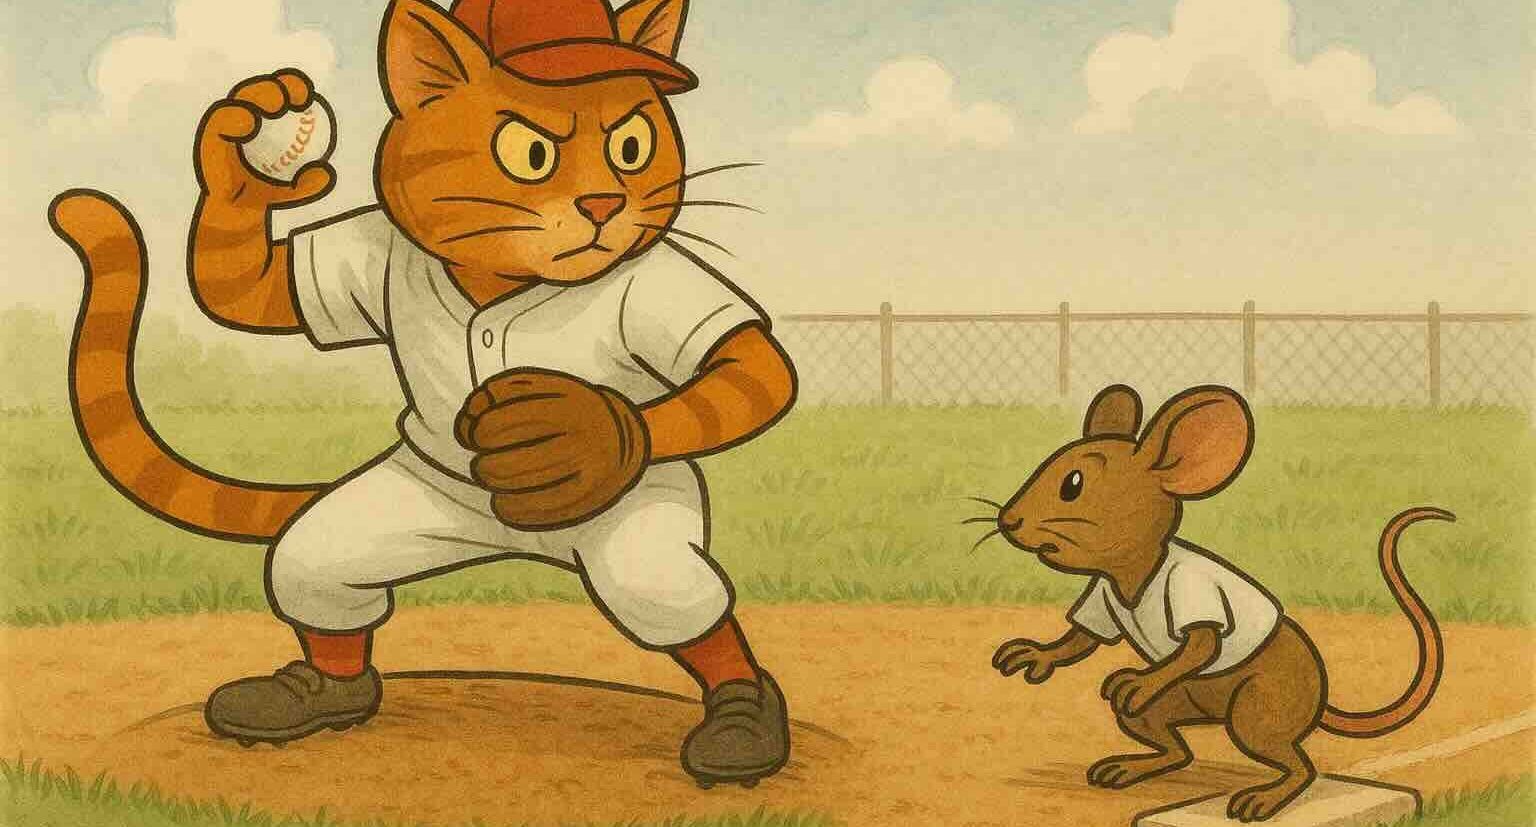
\includegraphics[width = 0.7\textwidth]{images/cat_and_mouse.jpg}
    \end{center}
    \hfill
    After \alert{\bf 3 failed pickoffs}, the runner advances automatically
  \end{frame}

  \begin{frame}{The Puzzle}
    How should the runner choose their lead distance to maximize \alert{\bf expected runs} scored in the inning?
    \vfill
    \hfill
    We got 2022--2023 \alert{\bf pitch-by-pitch lead distance} from MLB*\\
    \vfill
    \footnotesize \it *Major League Baseball trademarks and copyrights are used with permission of MLB Advanced Media, L.P. All rights reserved.
  \end{frame}

  \begin{frame}{Step 1: Estimate the effect of lead distance}
    How does lead distance influence\dots
    \begin{itemize}
      \item \alert{\bf Pickoff attempt} probability?
      \item \alert{\bf Pickoff success} probability?
      \item \alert{\bf Stolen base success} probability?
    \end{itemize}
    \vfill
    generalized linear mixed-effects model (GLMM)
    \begin{itemize}
      \item binomial likelihood for each outcome
      \item fixed effects: lead distance, disengagements, out, count, runner sprint speed, catcher arm strength
      \item random effects: pitcher, runner, catcher
    \end{itemize}
  \end{frame}

  \begin{frame}{Pickoff attempts increase with lead distance}
    \centering
    \includegraphics[width = 0.49\textwidth]{figures/prob_po_attempt_dark.pdf}
    \includegraphics[width = 0.49\textwidth]{figures/prob_po_success_dark.pdf}
  \end{frame}

  \begin{frame}{Stolen bases increase with lead distance}
    \includegraphics[width = \textwidth]{figures/prob_sb_success_dark.pdf}
  \end{frame}

  \begin{frame}{Step 2: Solve for the optimal lead distance policy}
    What is the \alert{\bf game-theoretic equilibrium} strategy?
    \vfill
    two-player sequential game
    \begin{itemize}
      \item state space: bases occupied, outs, count, disengagements
      \item action space: lead distance (runner), pickoff (pitcher)
      \item reward function: runs scored
      \item solved via \alert{\bf value iteration}
    \end{itemize}
  \end{frame}

  \begin{frame}{The Two-Foot Rule}
    \begin{columns}
      \begin{column}{0.5\textwidth}
        \centering
        \begin{tabular}{c|rrr}
          & \multicolumn{3}{c}{Disengagements}\\
          Count & 0 & 1 & 2\\
          \hline
          0-0 & 10.0 & 11.5 & 14.1 \\
          1-0 & 10.2 & 11.7 & 14.2 \\
          2-0 & 10.2 & 11.7 & 14.2 \\
          3-0 & 10.3 & 11.8 & 14.2 \\
          \hline
          0-1 & 9.8 & 11.4 & 14.1 \\
          1-1 & 10.0 & 11.6 & 14.2 \\
          2-1 & 10.3 & 11.8 & 14.3 \\
          3-1 & 10.4 & 11.9 & 14.3 \\
          \hline
          0-2 & 9.5 & 11.1 & 14.1 \\
          1-2 & 9.9 & 11.4 & 14.3 \\
          2-2 & 10.0 & 11.5 & 14.2 \\
          3-2 & 10.4 & 11.9 & 14.4
        \end{tabular}
      \end{column}
      \begin{column}{0.5\textwidth}
        \begin{itemize}
          \item Increase lead by \alert{\bf two feet} after each disengagement\\
          ~\\
          \item Value of implementation: $\sim$12 runs / team / season ($\sim$\$12,000,000)
        \end{itemize}
      \end{column}
    \end{columns}
  \end{frame}

  \begin{frame}{Should you just swing as hard as you can?}
    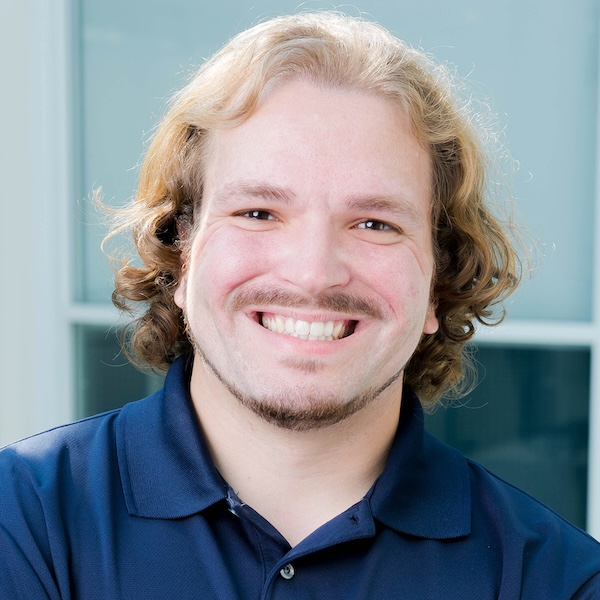
\includegraphics[height=0.5in]{images/collaborators/yurko.jpg}
    \alert{Ron Yurko}, Carnegie Mellon University\\
    ~\\
    \small Powers S, Yurko R (2026) ``Swinging, Fast and Slow: Interpreting variation in baseball swing tracking metrics''\\
    \href{https://arxiv.org/abs/2507.01238}{arXiv:2507.01238}, to appear in {\it The American Statistician}
  \end{frame}

  \begin{frame}{Background}
    Fans lament batters not having \alert{\bf two-strike approaches}
    \begin{center}
      \alert{\href{https://www.youtube.com/watch?v=SCG5sZtTpCc&t=909s}{(video)}}\\
      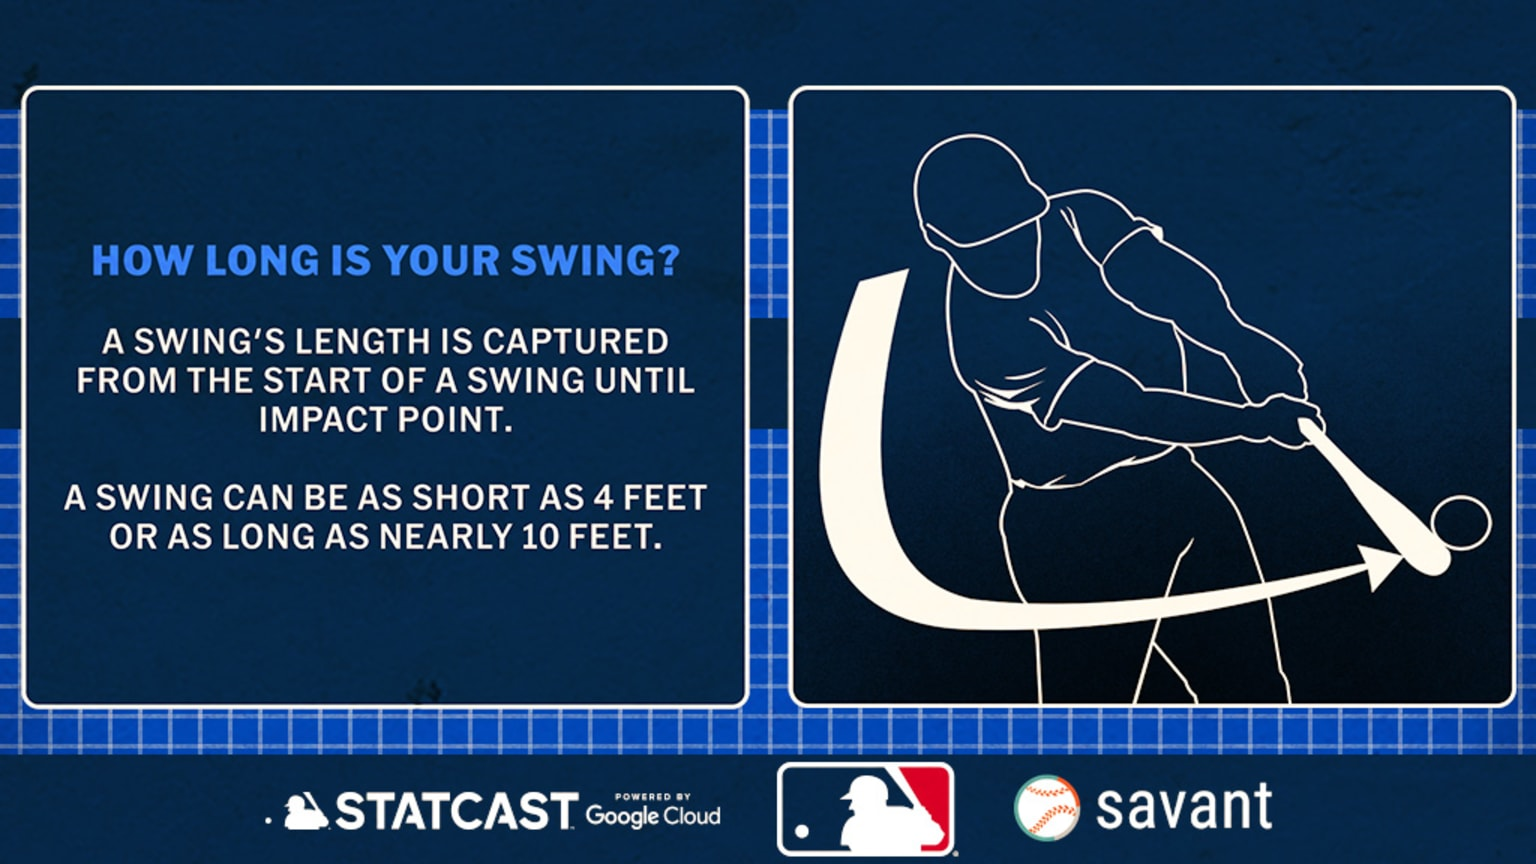
\includegraphics[width = 0.7\textwidth]{images/swing_length.jpg}
    \end{center}
    \hfill
    May 2024: MLB releases \alert{\bf swing length} and \alert{\bf bat speed} data
  \end{frame}

  \begin{frame}{Faster swings make better contact?}
    \begin{center}
      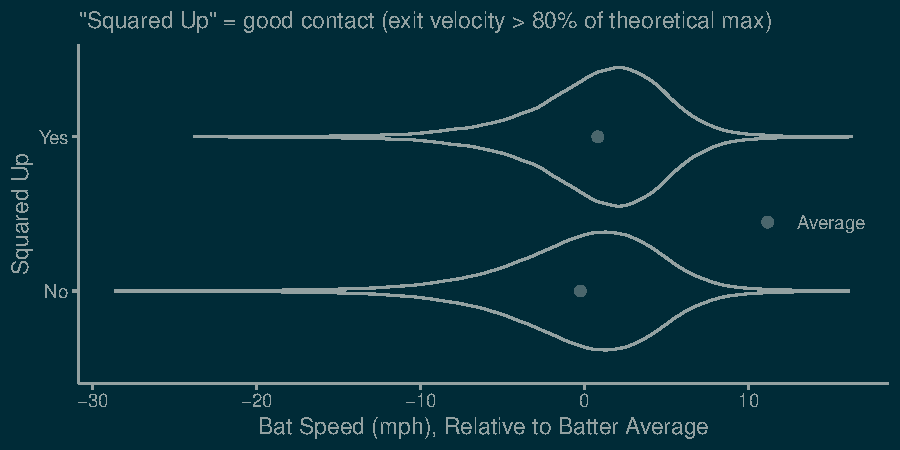
\includegraphics[width = \textwidth]{figures/counterintuitive.pdf}
    \end{center}
  \end{frame}

  \begin{frame}{Key Insight}
    We can't take swing metrics at \alert{\bf face value}
    \begin{center}
      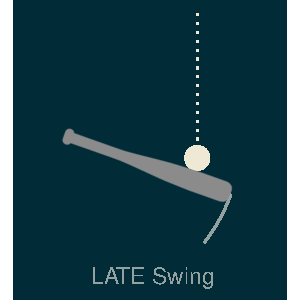
\includegraphics[width = 0.4\textwidth]{figures/swing_late.pdf}
      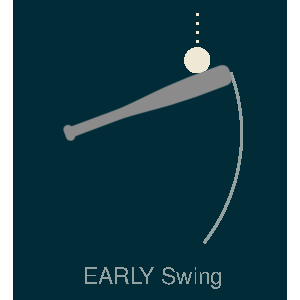
\includegraphics[width = 0.4\textwidth]{figures/swing_early.pdf}
    \end{center}
    \hfill
    Baseball Savant reports swing metrics at \alert{\bf point of contact}
  \end{frame}
  
  \begin{frame}{Step 1: Infer batter intention}
    What does the batter's swing look like\\
    \hfill
    \alert{\bf when they make solid contact?}\\
    \vfill
    Bayesian hierarchical model
    \begin{itemize}
      \item skew-normal likelihood for bat speed and swing length
      \item fixed effects: count, location
      \item random effects: batter, batter $\times$ count, batter $\times$ location
    \end{itemize}
  \end{frame}

  \begin{frame}{Some batters shorten/slow their swings more}
    \centering
    \includegraphics[height = 0.8\textheight]{figures/approach_dark.pdf}
  \end{frame}

  \begin{frame}{Step 2: Estimate effect of intention}
    If you make your swing \alert{\bf shorter/slower} with two strikes, do you make \alert{\bf more contact} with two strikes?\\
    \vfill
    Instrumental variables regression (causal inference)
    \begin{itemize}
      \item logistic regression for contact, linear regression for power
      \item instrument: count
      \item treatment: batter $\times$ count random effect
      \item control for difficulty of pitch (gradient boosting model)
    \end{itemize}
  \end{frame}

  \begin{frame}{Slower swings mean more contact, less power}
    \includegraphics[width = 0.49\textwidth]{figures/bat_speed_contact_dark.pdf}
    \includegraphics[width = 0.49\textwidth]{figures/bat_speed_power_dark.pdf}
  \end{frame}

  \begin{frame}{Step 3: Value the contact-power tradeoff}
    Is \alert{\bf increasing} your contact rate worth \alert{\bf decreasing} your power?\\
    \vfill
    Markov chain model
    \begin{itemize}
      \item state space: ball-strike count
      \item transition probabilities: depend on approach
      \item value function: linear weight of plate appearance outcome
    \end{itemize}
  \end{frame}

  \begin{frame}{The tradeoff is (roughly) balanced}
    \centering
    \includegraphics[height = 0.8\textheight]{figures/approach_run_value_dark.pdf}
  \end{frame}

  \begin{frame}{What does a pitch tell you about a pitcher?}
    \vfill
    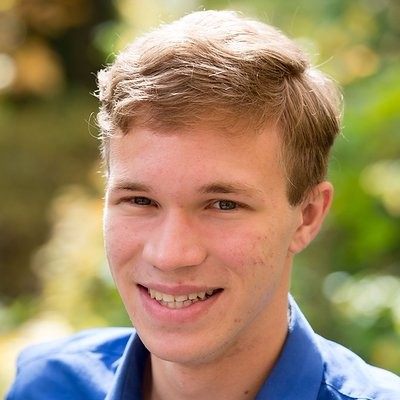
\includegraphics[height=0.5in]{images/collaborators/iglesias.jpg}
    \alert{Vicente Iglesias}, Susquehanna International Group\\
    ~\\
    Working paper:\\
    \small Powers S, Iglesias V ``Pitch trajectory density estimation for predicting future outcomes''
  \end{frame}

  \begin{frame}{Background}
    Full \alert{\bf pitch tracking} data have been available for 20 years
    \begin{center}
      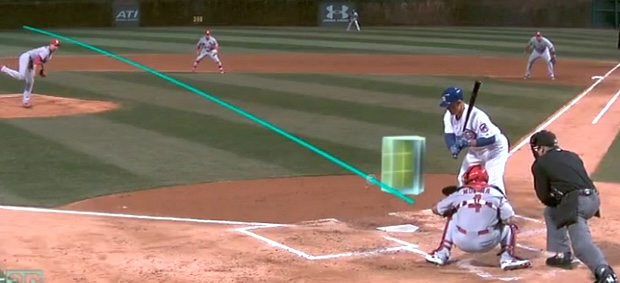
\includegraphics[width = 0.7\textwidth]{images/pitch_tracking.jpg}
    \end{center}
    \hfill
    Teams evaluate pitchers based on \alert{\bf pitches}, not outcomes\\
    \vfill
    \begin{center}
      \alert{\href{https://baseballsavant.mlb.com/sporty-videos?playId=c49715d9-1679-322e-b79d-01b397362c64}{(video \#1)}}
      \alert{\href{https://baseballsavant.mlb.com/sporty-videos?playId=3aa71fbe-65bb-33f7-8bde-f92a076e0227}{(video \#2)}}
    \end{center}
  \end{frame}

  \begin{frame}{Evaluating the {\it pitch} $\neq$ evaluating the {\it pitcher}}
    \begin{columns}
      \begin{column}{0.5\textwidth}
        \centering
        $\mbox{Variable Importance}^1$\\
        \includegraphics[width = \textwidth]{figures/feature_importance_dark.pdf}
      \end{column}
      \begin{column}{0.5\textwidth}
        \centering
        $\mbox{Variable Reliability}^2$\\
        \includegraphics[width = \textwidth]{figures/feature_reliability_dark.pdf}
      \end{column}
    \end{columns}
    \scriptsize
    \vfill
    ${}^1$ fractional contribution of each feature's splits to gradient boosting pitch model\\
    ${}^2$ (between-pitcher variance) / (total variance); varies by pitch type (here: RHB FB)
  \end{frame}

  \begin{frame}{Key Insight}
    \begin{columns}
      \begin{column}{0.4\columnwidth}
        \centering
        {\bf Supervised Learning}\\
        ~\\
        \begin{tabular}{ccc}
          Pitch &               & Outcome\\
          $x_1$ & $\rightarrow$ & $y_1$\\
          $x_2$ & $\rightarrow$ & $y_2$\\
          $x_3$ & $\rightarrow$ & $y_3$\\
                & ...           &      \\
          $x_n$ & $\rightarrow$ & $y_n$\\
          \\
          \\
          \\
          $x^*$ & $\rightarrow$ & $\hat y = \hat f(x)$\\
        \end{tabular}
      \end{column}
      \begin{column}{0.6\columnwidth}
        \centering
        {\bf Our Problem}\\
        ~\\
        \begin{tabular}{cccc}
          Pitcher & Pitch &               & Outcome\\
          A       & $x_1$ & $\rightarrow$ & $y_1$\\
          A       & $x_2$ & $\rightarrow$ & $y_2$\\
          B       & $x_3$ & $\rightarrow$ & $y_3$\\
                  &       & ...           &      \\
          C       & $x_n$ & $\rightarrow$ & $y_n$\\
                  & \\
                  &       & $\searrow$    & {\color{solarizedRebase03} $\int\hat p(x)\hat f(x)$}\\
                  & \\
          A       &  {\color{solarizedRebase03} $\hat p(x|\text{A})$}     &               & $\hat y$\\
        \end{tabular}
      \end{column}
    \end{columns}
  \end{frame}

  \begin{frame}{Key Insight}
    \begin{columns}
      \begin{column}{0.4\columnwidth}
        \centering
        {\bf Supervised Learning}\\
        ~\\
        \begin{tabular}{ccc}
          Pitch &               & Outcome\\
          $x_1$ & $\rightarrow$ & $y_1$\\
          $x_2$ & $\rightarrow$ & $y_2$\\
          $x_3$ & $\rightarrow$ & $y_3$\\
                & ...           &      \\
          $x_n$ & $\rightarrow$ & $y_n$\\
          \\
          \\
          \\
          $x^*$ & $\rightarrow$ & $\hat y = \hat f(x)$\\
        \end{tabular}
      \end{column}
      \begin{column}{0.6\columnwidth}
        \centering
        \alert{\bf Our Approach}\\
        ~\\
        \begin{tabular}{cccc}
          Pitcher & Pitch &               & Outcome\\
          A       & $x_1$ & $\rightarrow$ & $y_1$\\
          A       & $x_2$ & $\rightarrow$ & $y_2$\\
          B       & $x_3$ & $\rightarrow$ & $y_3$\\
                  &       & ...           &      \\
          C       & $x_n$ & $\rightarrow$ & $y_n$\\
                  & \\
                  & \alert{$\downarrow$}\\
                  & \\
          A       & \alert{$\hat p(x|\text{A})$} & \alert{$\rightarrow$} & \alert{$\int\hat p(x)\hat f(x)$}\\
        \end{tabular}
      \end{column}
    \end{columns}
  \end{frame}

  \begin{frame}{Step 1: Estimate distributions over pitch trajectories}
    What is the \alert{\bf generative model} for pitch trajectories?
    ~\\
    \vfill
    Bayesian hierarchical model
    \begin{itemize}
      \item multivariate normal likelihood (9 dimensions)
      \item mean $\sim$ pitcher, context, pitcher $\times$ context
      \item variance scaling $\sim$ pitcher, context
      \item correlation $\sim$ pitcher
    \end{itemize}
  \end{frame}

  \begin{frame}{Dylan Cease's Slider vs RHB in All Counts}
    \centering
    
\includegraphics[height = 0.85\textheight]{figures/656302_SL_R_plate.png}
  \end{frame}

  \begin{frame}{Step 2: Predict outcomes of pitch trajectories}
    What is the \alert{\bf run value} $\hat f(x)$ of each possible trajectory?\\
    \vfill
    gradient boosting
    \begin{itemize}
      \item predict run value of pitch
    \end{itemize}
    \vfill
    \begin{equation*}
      \text{predictive pitch score} = \int \left\{\hat p(x | \text{pitcher, context}) \cdot \hat f(x)\right\} dx
    \end{equation*}
  \end{frame}

  \begin{frame}{Predictive pitch score wins for $< 300$ pitches}
    \centering
    
\includegraphics[width = \textwidth]{figures/cor_by_sample_size.pdf}
  \end{frame}

  \begin{frame}{Thank You!}
    \begin{center}
      saberpowers.github.io\alert{/research}\\
    \end{center}
    \small
    ~\\
    Powers S, Ramani S, Hahn J, Schaefer AJ (2026)\\
    ``Lead distance under a pickoff limit in Major League Baseball: A sequential game model''\\
    \href{https://arxiv.org/abs/2601.15608}{arXiv:2601.15608}\\
    ~\\
    Powers S, Yurko R (2026)\\
    ``Swinging, Fast and Slow: Interpreting variation in baseball swing tracking metrics''\\
    \href{https://arxiv.org/abs/2507.01238}{arXiv:2507.01238}, to appear in {\it The American Statistician}\\
    ~\\
    Powers S, Iglesias V (working paper)\\
    ``Pitch trajectory density estimation for predicting future outcomes''
  \end{frame}

\end{document}
